\documentclass[12pt]{article}
\usepackage{amsmath}
\usepackage[english]{babel}
\usepackage{graphicx}
\usepackage{subfig}

\title{Detecting House Numbers in Street View Imagery using Convolutional Neural Networks}
\author{Matthew Peyrard}
\date{\today}

\begin{document}
\maketitle

\section{Definition}
\subsection{Project Overview}
Fully automated GPS and mapping services have become an indespensible part of our daily lives.
Keeping such services up to date is a very large task with a lot of available room for automation.
Cataloging house numbers from street view imagery is an important part of the mapping process.
The process of manually identifying and cataloging such imagery is very expensive due to the scale at which such a process must be applied.
However, if computational resources could be applied to the task with reasonably high accuracy, then the process could be sped up enormously, in addition to the costs saved from not having to hire thousands of people to perform the task manually.

In this project, I created a machine learning application that is capable of reading batches of images of street view house numbers, and outputting what numbers they are in a computer readable format.

\subsection{Problem Statement}
The goal of this project is to create an application that can be fed a collection of images containing house numbers and produce a prediction of what those house numbers are.
The tasks involved in solving this problem are the following:

\begin{enumerate}
	\item Download the \textit{Street View House Number} data set\cite{svhn_dataset}.
	\item Pre-process the data set into a more manageable form, for the sake of training speed and faster iteration. This is discussed in additional detail in Section \ref{sssec:data_exploration}.
	\item Train a logistic classifier (deep neural network) to recognize the digits in the training images.
	\item Build an application that uses the trained model to produce predictions from input imagery.
\end{enumerate}

The application is meant to be used for batch data on the command line, as the purpose is to automate the digit classification part of a street view ingest pipeline.

\subsection{Metrics}
Performance for this task is measured using an accuracy calculation based on a train/validation/test split.
In this case, the validation data is a random sample of 2000 entries from the training data.
The validation data is segregated from the rest of the training data, and only used to test performance periodically.
The performance of these periodic validation evaluations determines how we do checkpointing for the algorithm.
The model state is persisted to disk (checkpointed) whenever the performance of the model on the validation set has improved.

In this problem domain the output of the classifier is either correct, or it is not, therefore the accuracy is simply measured as the ratio of correct predctions to the total number of predictions.
Furthermore, no partial credit is provided for the algorithm, meaning that a prediction is correct if and only if all digits in the image are predicted correctly.

\section{Analysis}
\subsection{Data Exploration} \label{sssec:data_exploration}
The standard Street View House Number dataset\cite{svhn_dataset} was used for training and validation for this project. 
This data set comes with three sets of images: training, testing and extra. 
The training and testing data sets each consists of 33,402 and 13,068 images respectively. 
The extra dataset consists of over 200,000 images that are considered slightly easier, and are used as additional training and validation data. 
Each of these datasets also contains a \textit{Matlab} file that provides the labels and bounding boxes for each of the digits in each image.
For the purpose of this project, the Matlab file was converted into a CSV file that contained the image filename, digits and bounding boxes it contains. 
The Matlab file was scrapped because loading it took an excessive amount of time to load the data into memory.

\begin{figure}
\minipage{0.32\textwidth}
	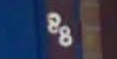
\includegraphics[width=\linewidth]{images/train/1046.png}
\endminipage\hfill
\minipage{0.32\textwidth}
	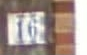
\includegraphics[width=\linewidth]{images/train/10.png}
\endminipage\hfill
\minipage{0.32\textwidth}
	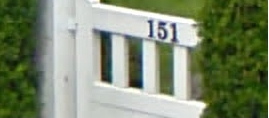
\includegraphics[width=\linewidth]{images/train/20.png}
\endminipage\hfill
\caption{Examples of SVHN imagery from the training set.}
\label{fig:example_imagery}
\end{figure}

\begin{figure}
\minipage{0.32\textwidth}
	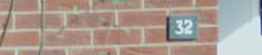
\includegraphics[width=\linewidth]{images/test/37.png}
\endminipage\hfill
\minipage{0.32\textwidth}
	
\includegraphics[width=\linewidth]{images/test/38.png}
\endminipage\hfill
\minipage{0.32\textwidth}
	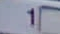
\includegraphics[width=\linewidth]{images/test/39.png}
\endminipage\hfill
\caption{Examples of SVHN imagery from the testing set.}
\label{fig:example_test_imagery}
\end{figure}

\begin{figure}
\minipage{0.32\textwidth}
	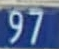
\includegraphics[width=\linewidth]{images/extra/140.png}
\endminipage\hfill
\minipage{0.32\textwidth}
	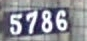
\includegraphics[width=\linewidth]{images/extra/148.png}
\endminipage\hfill
\minipage{0.32\textwidth}
	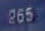
\includegraphics[width=\linewidth]{images/extra/156.png}
\endminipage\hfill
\caption{Examples of SVHN imagery from the extra set.}
\label{fig:example_extra_imagery}
\end{figure}

Figures \ref{fig:example_imagery} and \ref{fig:example_test_imagery} demonstrates some examples of the kinds of imagery we are dealing with in the SVHN dataset for training and testing. 
As you can see, there is a lot of variability in both the image size and image quality. 
For example in the center image, we can just barely tell that the first digit is a 1, but it could easily be misconstrued as a 7. 
However, one advantage that is provided by this data set is that digits, while not necessarily front and center, are at least prominent within the image.

Another potential complication is demonstrated by the left-most image, which shows that not all of the individual digits are lined up nicely.
Some of them are stacked diagonally or even vertically, and the neural network must be able to figure this out.

Many of these images are of relatively low quality, and present a considerable challenge to the neural network to learn.
However, as you can see from Figure \ref{fig:example_extra_imagery}, the imagery from the Extra data set is of considerably higher quality.
The digits are far less blurry, and tend to already take up the majority of the image.
This makes them much easier to work with because we will need far less resizing to bring the digits to the forefront of the image.

\subsection{Exploratory Visualization}
The first interesting property about the SVHN data set is the distribution of digit lengths across the different partitions (training, testing and extra).
Each image has one to five digits in the house number.
However, as shown in Figures \ref{fig:digit_length_plots} and \ref{fig:digit_length_table}, the digit lengths are not all equally represented by the training data.
This is likely representative of the relative probability of seeing a house number of each given length, but also raises the potential for the model to learn a bias towards common digit lengths, or against those less common ones.
As the data shows, digit lengths of two and three are far more common, while five digit house numbers are almost non-existent.

\begin{figure}[!htb]
\centering
\subfloat[Training\label{fig:train_digit_length_plot}]{
	\centering
	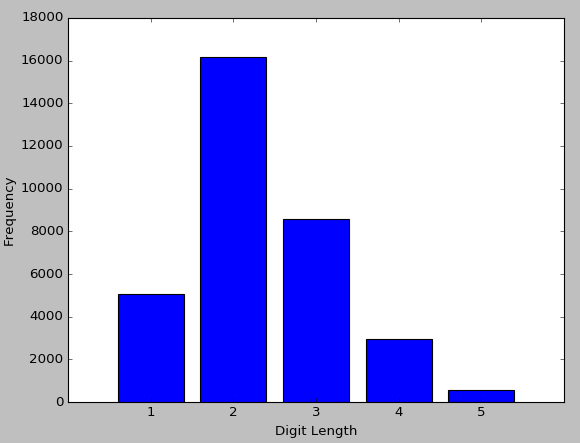
\includegraphics[width=0.45\columnwidth]{images/results/train_digit_lengths.png}
}\hfill
\subfloat[Testing\label{fig:test_digit_length_plot}]{
	\centering
	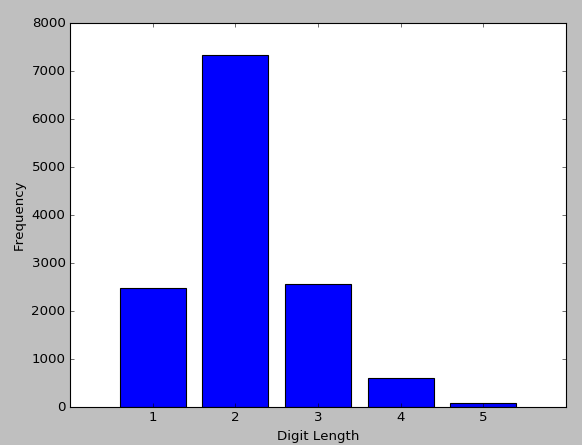
\includegraphics[width=0.45\columnwidth]{images/results/test_digit_lengths.png}
}\hfill
\subfloat[Extra\label{fig:extra_digit_length_plot}]{
	\centering
	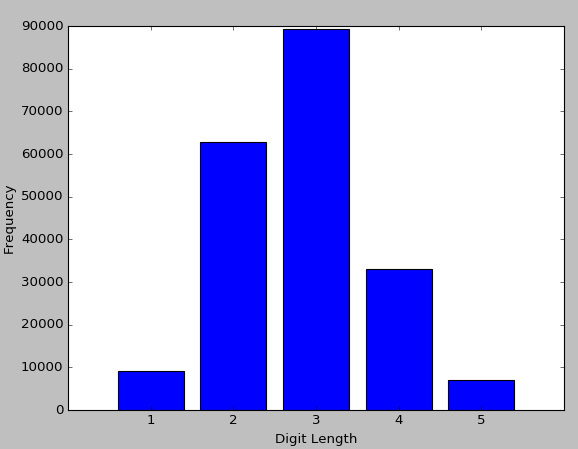
\includegraphics[width=0.45\columnwidth]{images/results/extra_digit_lengths.png}
}\hfill
\caption{Distributions of digit lengths for each of the training sets.}
\label{fig:digit_length_plots}
\end{figure}

\begin{figure}[!htb]
\begin{center}
\begin{tabular}{ |c|c|c|c|c|c| }
\hline
       & 1       & 2       & 3       & 4       & 5       \\
\hline
Train  & 15.25\% & 48.48\% & 25.69\% & 8.86\%  & 1.72\%  \\
\hline
Test   & 18.94\% & 56.13\% & 19.56\% & 4.67\%  & 0.70\%  \\
\hline
Extra  & 4.52\%  & 31.19\% & 44.36\% & 16.43\% & 3.48\%  \\
\hline
\end{tabular}
\end{center}
\caption{Ratio of each digit length's presence in its respective data set.}
\label{fig:digit_length_table}
\end{figure}

\begin{figure}[!htb]
\centering
\subfloat[Training\label{fig:train_digit_freq_plot}]{
	\centering
	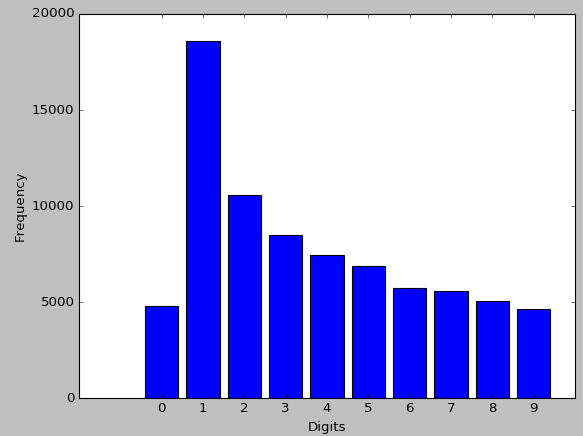
\includegraphics[width=0.45\columnwidth]{images/results/train_digit_freq.png}
}\hfill
\subfloat[Testing\label{fig:test_digit_freq_plot}]{
	\centering
	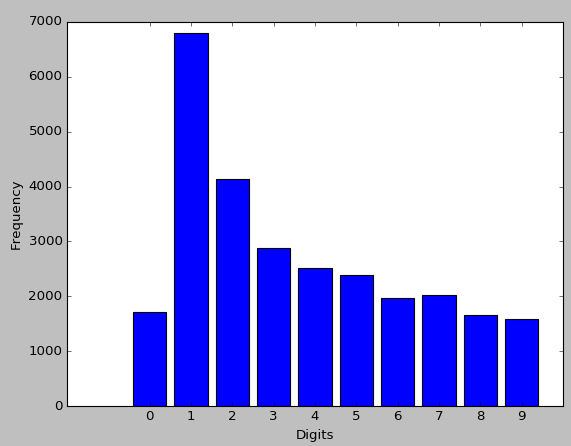
\includegraphics[width=0.45\columnwidth]{images/results/test_digit_freq.png}
}\hfill
\subfloat[Extra\label{fig:extra_digit_freq_plot}]{
	\centering
	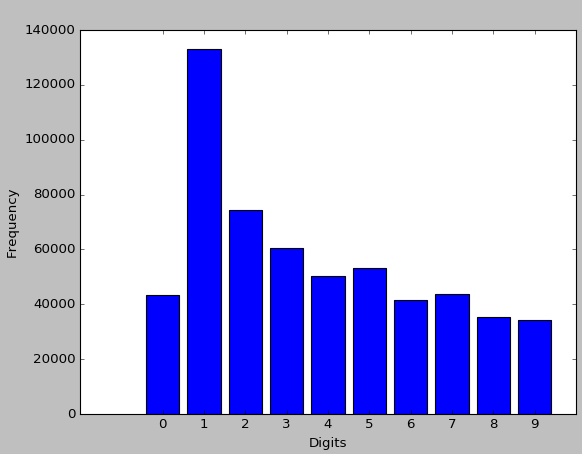
\includegraphics[width=0.45\columnwidth]{images/results/extra_digit_freq.png}
}\hfill
\caption{Distributions of individual digit frequencies for each of the training sets.}
\label{fig:digit_freq_plots}
\end{figure}

There is a similar asymmetry with the distribution of the individual digits.
As demonstrated by Figure \ref{fig:digit_freq_plots}, the digit 1 is by far the most common digit across all data sets.
Similar to the digit length bias, this asymmetry creates a potential bias towards the digit 1 in the model's predictions.
Even if there is not a bias, the model may be far more successful in recognizing 1's relative to other digits.

\subsection{Algorithms and Techniques}
In order to solve this problem, a convolutional neural network has been employed.
Convolutional neural networks are currently the most successful model employed for most computer vision problems.
For classification tasks, neural networks output a probability distribution representing their confidence in each class.
The prediction of the network is chosen as the label with the highest confidence probability score.

In this case, we have used an architecture similar to the one described in the original paper \cite{svhn_original_paper}, which means that we will have a unique softmax classifier for each digit in the house number.
This does, however, mean that there is a hard limit on the number of digits that can be recognized by the model.
As in the original paper, I have chosen that limit to be five.
One divergance from the original paper is the lack of a length prediction classifier.
In the original paper, if a house number was less than five digits long, then the prediction would have random predictions for the stranded digits.
This was remedied by a sixth classifier output that would provide the digit length, thereby allowing you to determine which digits were true predictions.

While this approach was tested during this project, superior results were achieved by discarding the length prediction and simply introducing a placeholder digit class to signify that the digit does not exist in the picture.
This approach yielded results superior to the length prediction strategy.

This algorithm contains several hyper-parameters:

\begin{itemize}
	\item The optimization algorithm $\mathcal{O}$ is responsible for using the output of the loss function $\mathcal{L}$ to update the weights of the neural network. Several different algorithms were tested, including Adam, Adagrad and Adadelta. $\mathcal{O}$ also has several hyper-parameters of its own:
	\begin{itemize}
	\item While the optimizer $\mathcal{O}$ determines the relative distribution of the updates to the weights in the network, the learning rate $\alpha$ determines how large those updates end up being.
	\item The use of exponential decay introduces several other parameters: the initial learning rate $\alpha_0$, the number of epochs $\varepsilon$ over which the decay takes place, and the final learning rate $\alpha_{\varepsilon-1}$.
	\end{itemize}

	\item The neural network architecture:
	\begin{itemize}
		\item The number of layers in the neural network. This has a direct impact on the number of parameters used in the model.
		\item The number of filters in each convolutional layer.
		\item The receptive field size in each convolutional layer.
		\item The stride and padding of the convolutional layers.
		\item The size of the fully connect layers (in terms of units).
		\item The training dropout rate.
		\item The stride and padding of the max-pooling layers.
	\end{itemize}

	\item Input normalization parameters:
	\begin{itemize}
		\item The use of statistical centering techniques, such as mean subtraction or variance normalization.
		\item Input image size.
	\end{itemize}
\end{itemize}

Once loaded and normalized, the training data is randomly sampled in batches of 64 and run through the neural network and its optimizer.
Backpropagation of the loss $\mathcal{L}$ is done using the Adagrad optimizer.

Every 100 iterations the validation set is run through the network and its accuracy measured and recorded.
If the performance on the validation set is the best seen thus far, then  the model is checkpointed to disk so that it can be restored later and used in production.
This process continues until no improvement is observed for several hours (no hard limit was set).
The best performing model (according to the performance on the validation set) is then used for testing and production.

All training and testing was done on a GPU using TensorFlow version 0.10.


\subsection{Benchmark}
The primary benchmark used for this project was from the original paper \cite{svhn_original_paper}, where they cite 96\% accuracy on the SVHN data set. As this is my first deep learning project, I set the goal of achieving over 85\% accuracy on the testing set.

\section{Methodology}
\subsection{Data Preprocessing}
Upon initialization of the training algorithm, the training data is loaded from disk into memory.
The data is then split into training and validation sets.
The split is performed by first randomly shuffling the data, and then randomly sampling 2,000 examples and setting them aside as the validation set.

Following this step, the images are cropped based on the bounding boxes from the training file (CSV) and then resized to a $32 \times 32 \times 3$ numpy array.
The images are cropped in order to make sure the digits are front and centre.
This helps the learning algorithm identify the digits better by reducing the amount of noise it has to deal with.
In reality we would not be dealing with such convenient imagery, but this step is used as a placeholder for localization techniques that are beyond the scope of this project.

Following the cropping step, the mean $\mu_t$ of all of the pixels in all of the training images (not from the validation set) is computed and stored to disk. 
$\mu_t$ is then subtracted element-wise from all of the pixels in the training and validation sets as a normalization step.
The training mean is stored to disk because it must also be subtracted from any images we run as part of the testing or in production, since the model will be trained with such a normalization in mind.

\subsection{Implementation}


\subsection{Refinement}
The biggest sources of improvement during this project was the adjustment of the learning rate and increasing the size of the network.
The network was initially half the size of the final architecture, with four convolutional layers, and one fully connected layer.
The learning rate was initially set statically to 0.05, which was good enough to get the model off the ground, but it often got stuck at around 40\% accuracy. 
Such a learning rate was clearly too high to allow the optimizer to find the smaller crevices that lead to higher accuracies. 
In response to this, some major performance improvements were gained by lowering the learning rate to 0.025 and introducing the exponential decay.
This allowed the accuracy to increase to 80\%, however once it reached this point, the network would suddenly jump out of its current optimum, and land somewhere completely sub-optimal. 
This can be seen in Figure \ref{fig:small_network_results}.
Whether this was a Tensorflow bug, or as a result of a flawed architecture, was not discernable.
However, by increasing the network size, in addition to the changes in the learning rate, the accuracy (on the validation set) was able to exceed 90\%. 
Those results are discussed in Section \ref{sssec:justification}.

There were two methods for this, the most successful of which has been outlined in Section \ref{sssec:evaluation}.
The second method was the one described in the original paper \cite{svhn_original_paper}, which uses length prediction in place of placeholder digits.
The length prediction method was attempted and achieved a 90.1\% validation accuracy, which is shown in Figure \ref{fig:length_best_results}.
This result was impressive, but the result of 96\% using placeholder digits easily eclisped it.

\begin{figure}[!htb]
\centering
\subfloat[Loss\label{fig:lenth_best_loss}]{
	\centering
	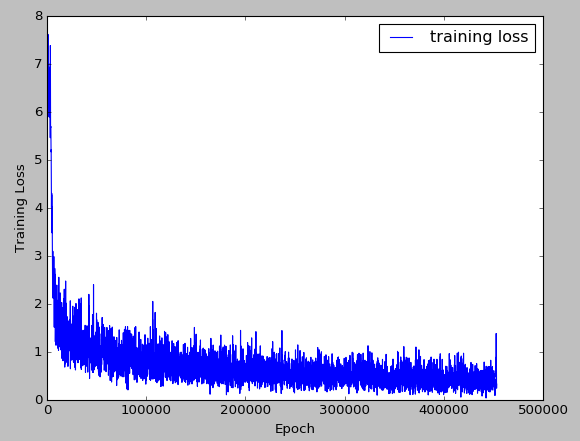
\includegraphics[width=0.45\columnwidth]{images/results/length_best_loss.png}
}\hfill
\subfloat[Accuracy\label{fig:length_best_accuracy}]{
	\centering
	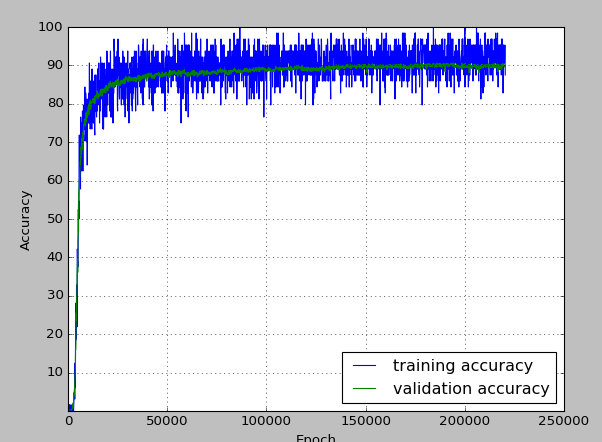
\includegraphics[width=0.45\columnwidth]{images/results/best_accuracy.png}
}\hfill
\caption{Plot of best run using length prediction, $\alpha_0 = 0.025$, 50,000 epoch decay to 0.0075.}
\label{fig:length_best_results}
\end{figure}

\begin{figure}[!htb]
\centering
\subfloat[Loss\label{fig:small_best_loss}]{
	\centering
	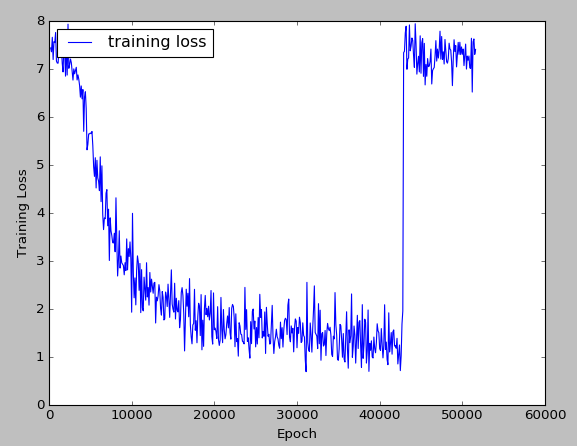
\includegraphics[width=0.45\columnwidth]{images/results/small_network_loss.png}
}\hfill
\subfloat[Accuracy\label{fig:small_best_accuracy}]{
	\centering
	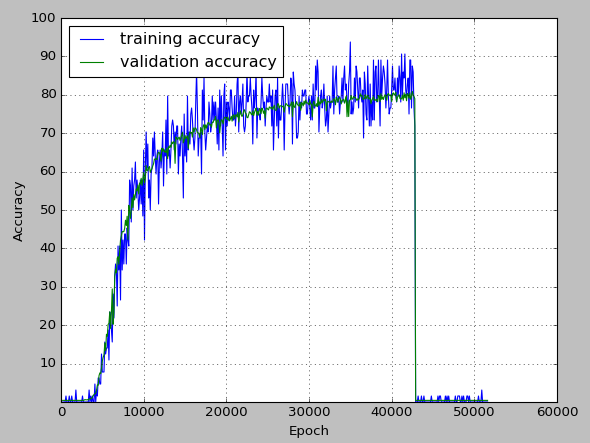
\includegraphics[width=0.45\columnwidth]{images/results/small_network_accuracy.png}
}\hfill
\caption{Plot of run using smaller convolutional network, $\alpha_0 = 0.025$, 30,000 epoch decay to 0.001.}
\label{fig:small_network_results}
\end{figure}



\section{Results}
\subsection{Model Evaluation and Validation} \label{sssec:evaluation}
The final architecture of the neural network is roughly based on the design outlined in the original paper \cite{svhn_original_paper}.
The network uses eight convolutional layers, with depths of 48, 64, 128 and 160 for the first four layers, and 192 for the final four layers.
This is followed by two fully connected layers with 4096 units each.
The network then splits into five output layers, each one predicting one of the up-to-five digits in the image. 
Each output layer is assigned a static index $i$, and that layer is responsible for predicting the $i$-th digit. 
If the number has fewer digits than $i$, then the output layer will output the null class, which in this case is just the digit 10.
Each output layer is a fully connected softmax classifier.

Every convolutional layer and pre-output fully connected layer uses ReLU\cite{relu} activations followed by dropout\cite{svhn_dropout} and local response normalization\cite{svhn_lrn} layers.
The convolutional kernel size for all convolutional layers was $5 \times 5$, along with a stride of 1.

Max pooling was used twice, once following convolutional layer 4, and again following convolutional layer 8.
Both max pooling layers used $2 \times 2$ windows with a stride of 1.

The Adagrad optimizer was used with exponential decay. I used an initial learning rate $\alpha_0 = 0.025$, decaying over the course of 50,000 epochs to a final learning rate of 0.001.

\subsection{Justification} \label{sssec:justification}
For this evaluation, two different models were used.
For the first model, only the training set was used for training, and achieved a validation accuracy of 89.9\% and a training accuracy of 82.7\%, which falls short of the 85\% goal I set for myself.
These results are shown in Figure \ref{fig:final_lessdata}.
However, the same model's accuracy when testing on the extra data set (which was not used for any kind of training) achieved 95.8\% accuracy.
The second model used both the training and extra sets for training, and achieved a validation accuracy of 96\% and a test accuracy of 88.8\% on the test set.
These results are shown in Figure \ref{fig:final_moredata}.

\begin{figure}
\centering
\subfloat[Loss\label{fig:final_loss_lessdata}]{
	\centering
	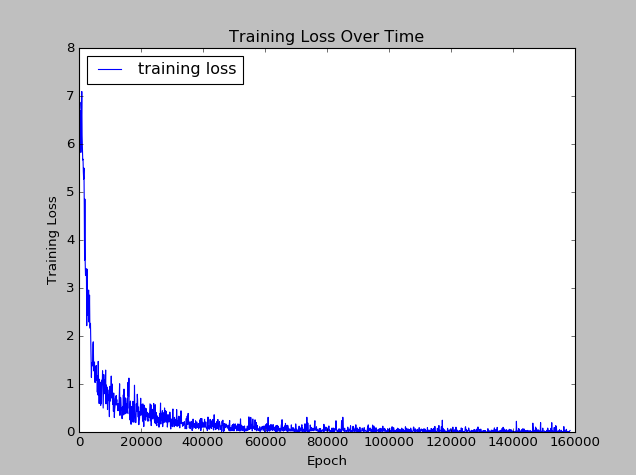
\includegraphics[width=0.45\columnwidth]{images/results/train_loss_lessdata.png}
}\hfill
\subfloat[Accuracy\label{fig:final_accuracy_lessdata}]{
	\centering
	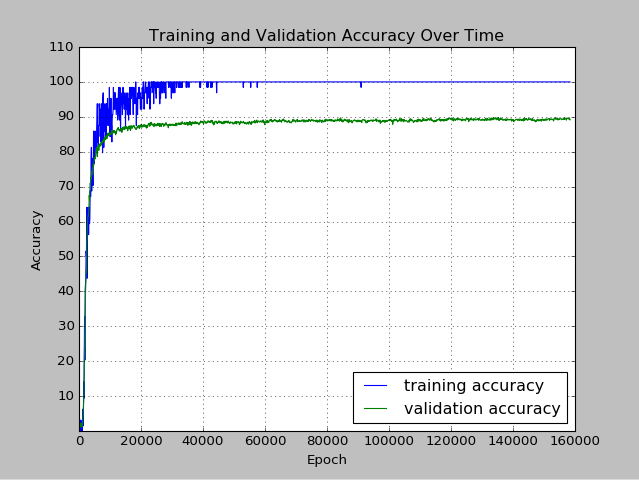
\includegraphics[width=0.45\columnwidth]{images/results/accuracy_lessdata.png}
}\hfill
\caption{Plot of run using smaller convolutional network, $\alpha_0 = 0.025$, 50,000 epoch decay to 0.001. Trained using just the training set.}
\label{fig:final_lessdata}
\end{figure}

\begin{figure}
\centering
\subfloat[Loss\label{fig:final_loss_moredata}]{
	\centering
	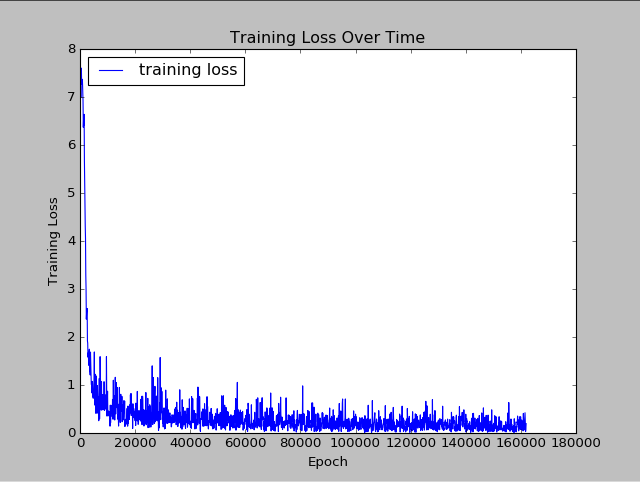
\includegraphics[width=0.45\columnwidth]{images/results/training_loss_moredata.png}
}\hfill
\subfloat[Accuracy\label{fig:final_accuracy_moredata}]{
	\centering
	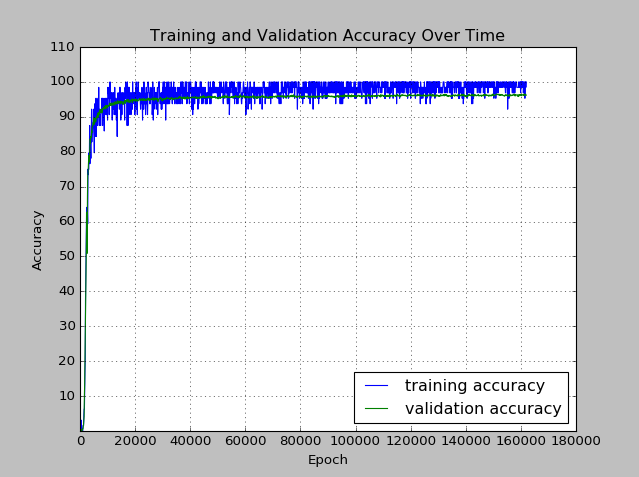
\includegraphics[width=0.45\columnwidth]{images/results/accuracy_moredata.png}
}\hfill
\caption{Plot of run using smaller convolutional network, $\alpha_0 = 0.025$, 50,000 epoch decay to 0.001. Trained using the union of training and extra sets.}
\label{fig:final_moredata}
\end{figure}

\section{Conclusion}
\subsection{Free-Form Visualization}
\subsection{Reflection}
\subsection{Improvement}


\begin{thebibliography}{9}
\bibitem{svhn_dataset} 
Yuval Netzer, Tao Wang, Adam Coates, Alessandro Bissacco, Bo Wu, Andrew Y. Ng 
\textit{Reading Digits in Natural Images with Unsupervised Feature Learning NIPS Workshop on Deep Learning and Unsupervised Feature Learning 2011.}
http://ufldl.stanford.edu/housenumbers/
\bibitem{svhn_original_paper}
Goodfellow, Ian J.; Bulatov, Yaroslav; Ibarz, Julian; Arnoud, Sacha; Shet, Vinay
\textit{Multi-digit Number Recognition from Street View Imagery using Deep Convolutional Neural Networks}
\bibitem{svhn_lrn}
Alex Krizhevsky and Sutskever, Ilya and Geoffrey E. Hinton
\textit{ImageNet Classification with Deep Convolutional Neural Networks}
\bibitem{svhn_dropout}
Nitish Srivastava, Geoffrey Hinton, Alex Krizhevsky, Ilya Sutskever, Ruslan Salakhutdinov
\textit{Dropout: A Simple Way to Prevent Neural Networks from Overfitting}
\bibitem{relu}
R Hahnloser, R. Sarpeshkar, M A Mahowald, R. J. Douglas, H.S. Seung (2000). 
\textit{Digital selection and analogue amplification coesist in a cortex-inspired silicon circuit.}

\end{thebibliography}
	
\end{document}

